 \documentclass{jacow}
\usepackage{graphicx}
\usepackage{booktabs}
\usepackage{bigints}
\usepackage{url}
\usepackage{grffile} % can use other graphics extensions (e.g. doesn't error for example.0.1.png)
\usepackage{float} % \begin{figure}[H] makes figures not float (really really here)
\usepackage{array}
\usepackage{cite}
\newcolumntype{P}[1]{>{\centering\arraybackslash\vspace{-2mm}}p{#1}}


\usepackage{svg}
%%
%%   VARIABLE HEIGHT FOR THE TITLE BOX (default 35mm)
%%

\setlength{\titleblockheight}{35mm}

\begin{document}
\title{Hybrid Methods for Simulation of Muon Ionization Cooling Channels\thanks{Work supported by the U.S. Department of Energy}}

\author{J. Kunz, Illinois Institute of Technology, Chicago, IL, USA \\
P. Snopok\thanks{psnopok@iit.edu}, Illinois Institute of Technology, Chicago, IL, USA and Fermilab, Batavia, IL, USA \\
M. Berz, K. Makino, Michigan State University, East Lansing, MI, USA}

\maketitle

\begin{abstract}
COSY Infinity is an arbitrary-order beam dynamics simulation and analysis code. It can determine high-order transfer maps of combinations of particle optical elements of arbitrary field configurations. For precision modeling, design, and optimization of next-generation muon beam facilities, its features make it a very attractive code. New features are being developed for inclusion in COSY to follow the distribution of charged particles through matter. To study in detail some of the properties of muons passing through material, the transfer map approach alone is not sufficient. The interplay of beam optics and atomic processes must be studied by a hybrid transfer map--Monte Carlo approach in which transfer map methods describe the average behavior of the particles in the accelerator channel including energy loss, and Monte Carlo methods are used to provide small corrections to the predictions of the transfer map accounting for the stochastic nature of scattering and straggling of particles. The advantage of the new approach is that it is very efficient in that the vast majority of the dynamics is represented by fast application of the high-order transfer map of an entire element and accumulated stochastic effects as well as possible particle decay. The gains in speed are expected to simplify the optimization of muon cooling channels which are usually very computationally demanding due to the need to repeatedly run large numbers of particles through large numbers of configurations. Progress on the development of the required algorithms is reported.
\end{abstract}

\section{INTRODUCTION}

Muons are typically tertiary production particles (protons $\rightarrow$ pions $\rightarrow$ muons) and high-intensity collection requires a large initial phase space volume. The resultant spray of muons must be amassed, focused, and accelerated well within the muon lifetime (2.2~$\mu$s in the rest frame). The only technique fast enough to reduce the beam size within the muon lifetime is ionization cooling. When muons traverse a material, energy is lost in both the longitudinal and transverse directions due to ionization. The energy is then restored in the longitudinal direction only, leading to an overall reduction in the transverse beam size (cooling). In order to achieve cooling in the longitudinal direction, emittance exchange is used, usually involving wedge-shaped absorbers. For some applications such as a high-energy high-luminosity muon collider, cooling needs to be very aggressive: six-dimensional emittance reduction over six orders of magnitude is required to reach design goals.

In order to carefully simulate the effect of the absorbers on the beam, one needs to take into account both deterministic and stochastic effects in the ionization energy loss. The deterministic approach relying on the Bethe-Bloch formula with various theoretical and experimental corrections fits well into the transfer map methods approach, where the effect of the lattice on the particles is evaluated first by producing the so-called transfer map, that is then applied to a given initial distribution of particles. The arbitrary-order simulation code COSY Infinity \cite{COSY} is a key representative of transfer map codes. COSY was chosen because of its built-in optomization tools, speed, its ability to produce high-order transfer maps, and its ability to control individual aberrations. 

However, to take into account stochastic effects the transfer map paradigm needs to be augmented by implementing the corrections from stochastic effects directly into the fabric of COSY. Some of the fundamental ideas of the process were presented in~\cite{errede} in application to quadrupole cooling channels, but the approximations used were fairly basic. In this work, a more rigorous theoretical approach is used, and the resulting valiation is presented. 

\section{Cooling Absorbers in COSY Infinity}
Recently, support for matter-dominated lattices has been implemented into COSY \cite{ipac2015}, with the application of cooling absorbers as the motivation. Excellent agreement has been achieved between COSY, G4Beamline \cite{G4BL}, and ICOOL \cite{icool} for pencil beams of varying momenta through varying liquid hydrogen absorber lengths. The ranges which have been tested are $(p,L)$ combinations of $p=(100,200,300,400)$ MeV/$c$ and $L=(1,10,100)$ mm. The combination of $(p,L)=(200\text{ MeV/}c, 100\text{ mm})$ is presented in Figure \ref{fig:LH_validation}, as this is a typical regime of cooling absorbers.

\begin{figure}[!ht]
\centering
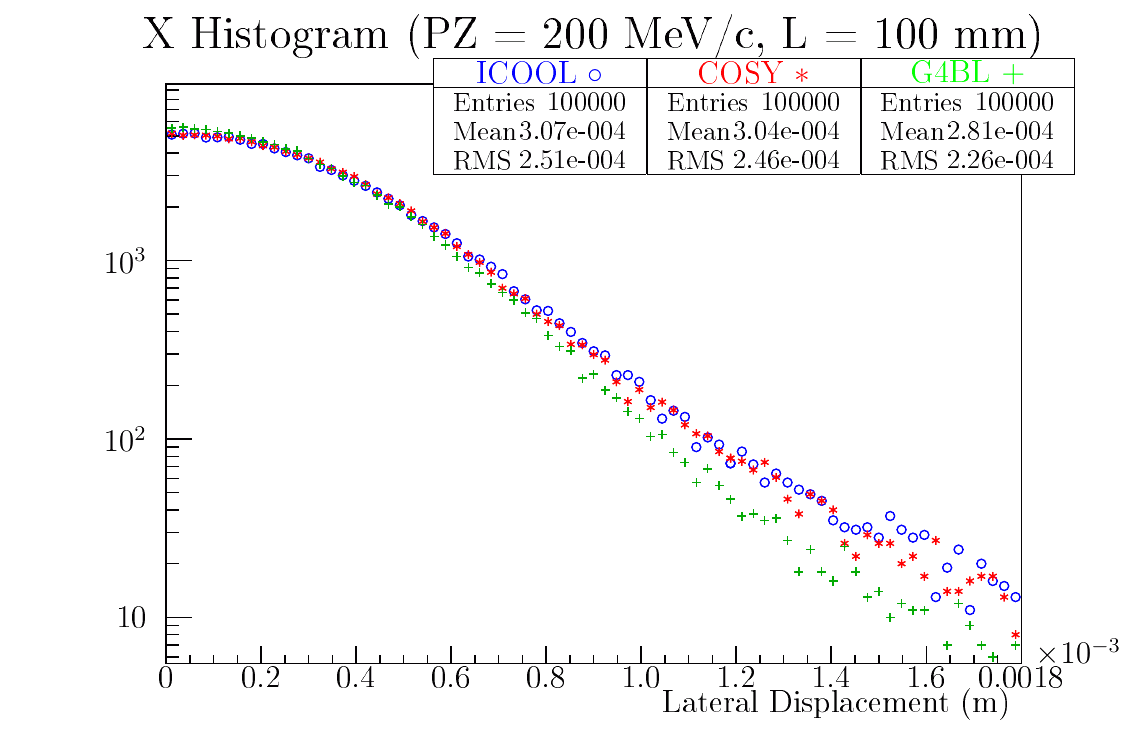
\includegraphics[width=\columnwidth]{LH.X.200.100.png}
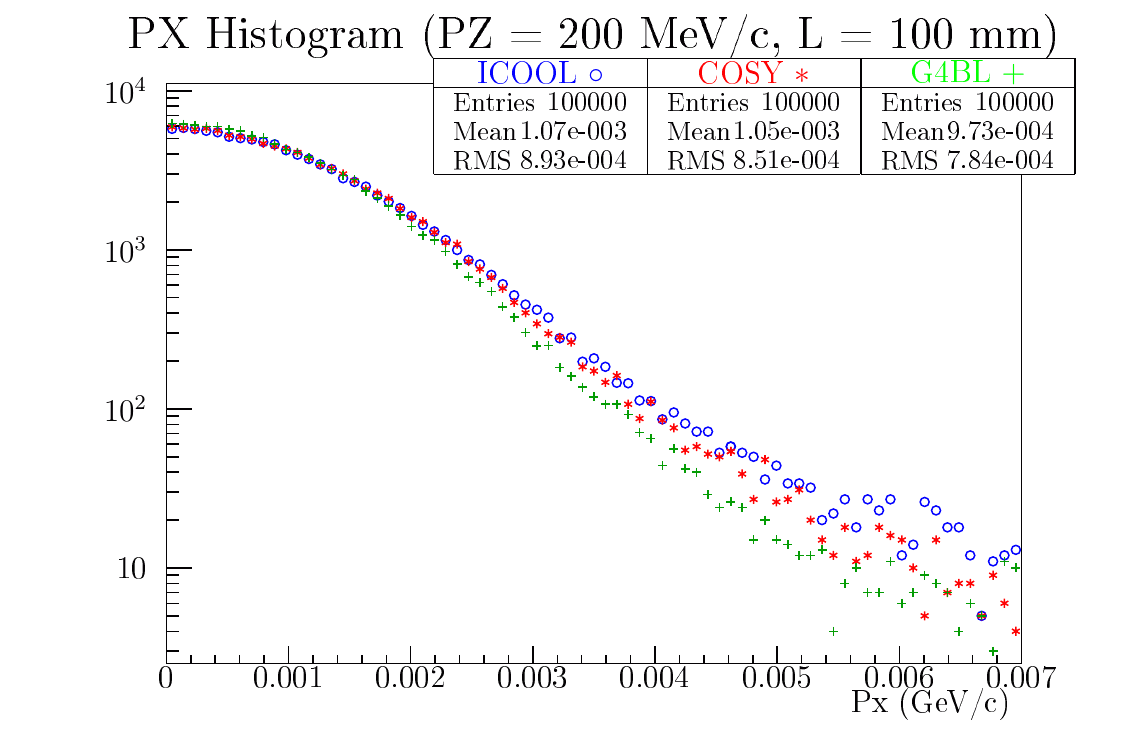
\includegraphics[width=\columnwidth]{LH.PX.200.100.png}
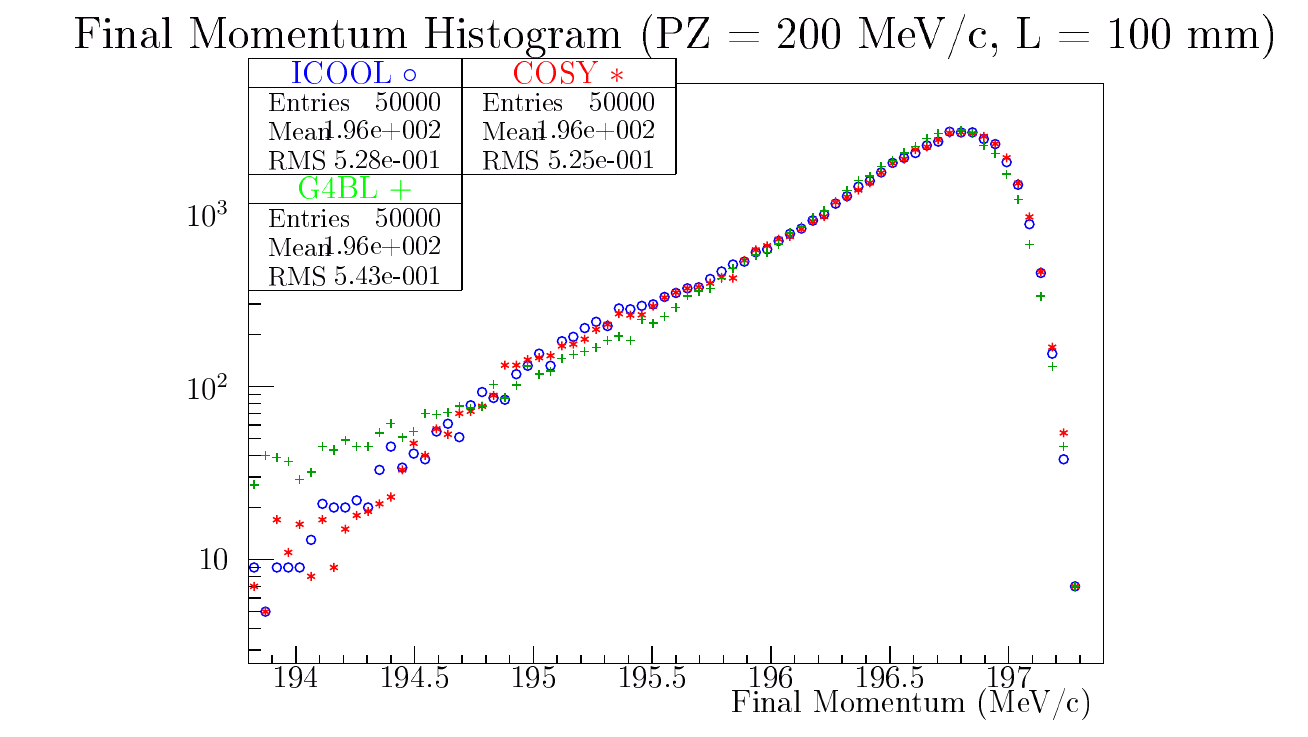
\includegraphics[width=\columnwidth]{LH.strag.200.100.png}
\caption{Comparison between COSY, G4beamline, and ICOOL for a 200 MeV/$c$ pencil beam passing through 100~mm of liquid hydrogen. Position (top), transverse momentum (middle), final total momentum (bottom) histograms.}
\label{fig:LH_validation}
\end{figure}

Moreover, COSY has been compared to the experimental results of the Muon Scattering Experiment \cite{muscat}. Agreement has been shown for Be @ 3.73 mm, LH @ 159 mm, and LH @ 109 mm, with the last result reproduced in Figure \ref{fig:muscat}.

\begin{figure}[!ht]
\centering
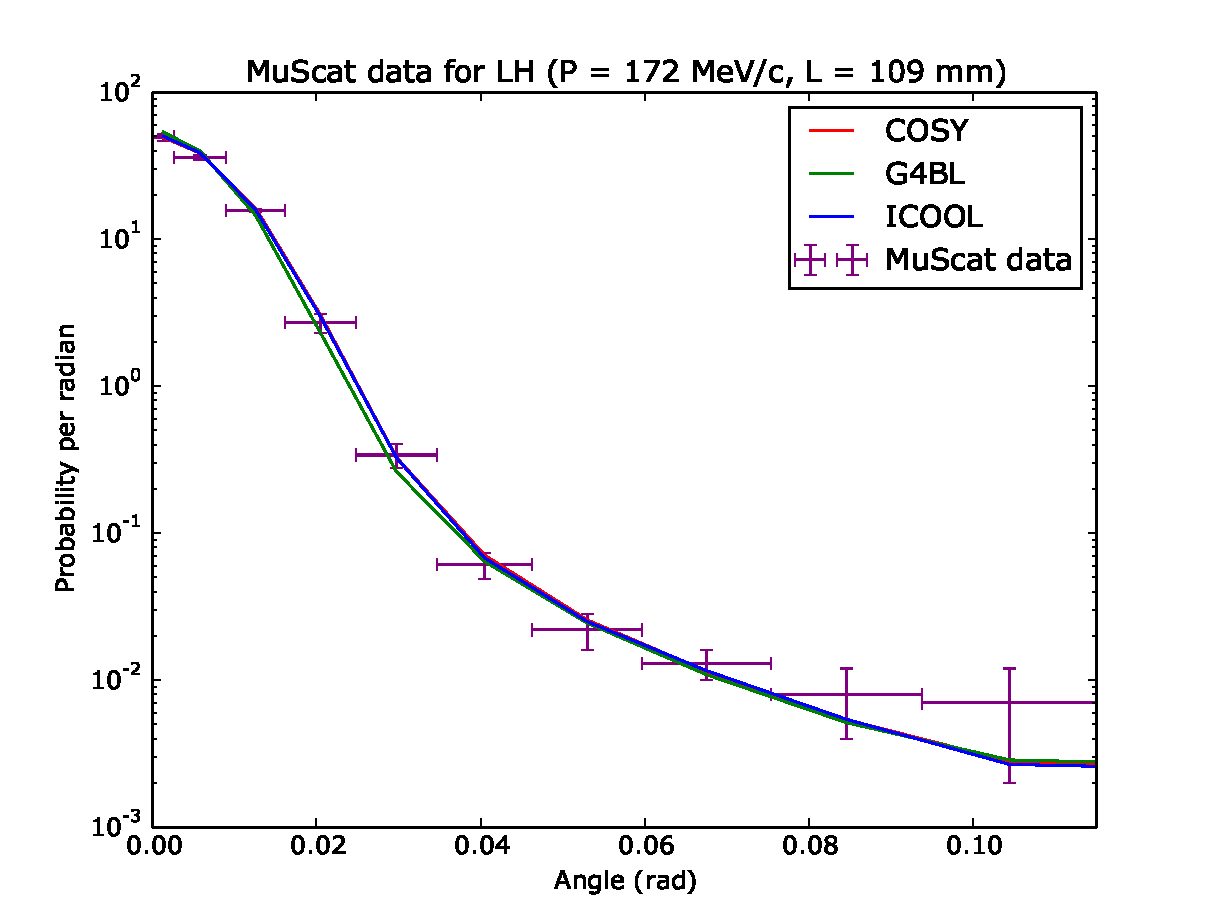
\includegraphics[width=0.9\columnwidth]{172.109.muscat.pdf}
\caption{Comparison of COSY, G4beamline, and ICOOL with MuScat experiment results.}
\label{fig:muscat}
\end{figure}

\section{The Muon Ionization Cooling Experiment}
The international Muon Ionization Cooling Experiment (MICE)~\cite{mice} at Rutherford Appleton Laboratory will demonstrate muon cooling by reducing the emittance of a muon beam and measuring it with an accuracy of 0.1\%. MICE is implemented in steps. Step IV is currently taking data. This is the first ionization cooling demonstration without reacceleration. Step IV tests beam propagation in the magnetic system and allows precise measurement of ionization cooling related properties of absorbers (liquid hydrogen and LiH). The cell of Step IV includes 12 solenoidal coils which are symmetric about an absorber. In this study we use a flat, 65~mm lithium hydride absorber (Figure~\ref{fig:mice_channel}).
%
\begin{figure}[!ht]
\centering
\includegraphics*[width=\columnwidth]{mice_channel.png}
\caption{MICE Step IV channel magnetic coils (yellow) and LiH absorber (gray)in the center.}
\label{fig:mice_channel}
\end{figure}

The MICE simulation was carried out in both COSY and G4Beamline in parts, absorber effect and magnetic field effect separately. The initial distribution parameters are summarized in Table~\ref{tbl:initial_distribution}. First, the coils were tested in either code. In G4Beamline, the coils were realized using the \texttt{coil} and \texttt{solenoid} routines with the parameters in Table~\ref{tbl:coil_parameters}. These routines approximate each cylindrical coil by a number of thin sheets. The number of sheet is based on the prescribed tolerance characterizing the maximum error in the field. The same coil geometry was used in COSY. Here, the 11$^\text{th}$ order transfer map of the coils was created using the built-in \texttt{CMSTP} routine that uses the on-axis field and out-of-axis expansion. The initial distribution was then propagated through this map. These results are summarized in Figure~\ref{fig:mice_coil_histograms}.

\begin{table}[!ht]
\begin{center}
%\hspace*{-0.6cm}
%\vspace*{-0.5cm}    
\caption{Initial beam parameters for MICE Step IV simulation.}
\begin{tabular}{cc}
	\toprule
	\textbf{Parameter} & \textbf{Value}\\ 
	\midrule
	Type & Gaussian on-axis\\
	Total count & $10^4$\\
	$\sigma_x, \sigma_y$ & 32 mm\\
	$\sigma_{P_x}, \sigma_{P_y}$ & 19 MeV/c\\
	$\sigma_{P_z}$ & 29 MeV/\textit{c} \\
	$P_z$ & 200 MeV/\textit{c} \\
	\bottomrule
\end{tabular}
\label{tbl:initial_distribution}
\end{center}
\end{table}

\begin{table}[!ht]
\small
\begin{center}
\caption{Coil parameters for MICE Step IV simulation.}
\begin{tabular}{cccccc}
	\toprule
	\textbf{Coil} & \textbf{z} & \textbf{Length} & \textbf{Inner} & \textbf{Outer} & \textbf{Current}\\
	\textbf{name} & & & \textbf{radius} & \textbf{radius} & \textbf{density}\\
	 & \textbf{(mm)} & \textbf{(mm)} & \textbf{(mm)} & \textbf{(mm)} & \textbf{(A/mm$^2$)}\\
	\midrule
	End2 & $\mp$3200&111&258&326&$\pm$126 \\
	Center&$\mp$3250&1314&258&280&$\pm$148 \\
	End1 & $\mp$1700 & 111& 258 & 319 & $\pm$133 \\
	Match2 & $\mp$1300 & 199 & 258 & 289 & $\pm$132 \\
	Match1 & $\mp$861 & 201 & 258 & 304 & $\pm133$ \\
	Focus & $\mp$202 & 213 & 268 & 362 & $\pm$104 \\
	\bottomrule
\end{tabular}
\label{tbl:coil_parameters}
\end{center}
\end{table}

\begin{figure}[!ht]
\centering
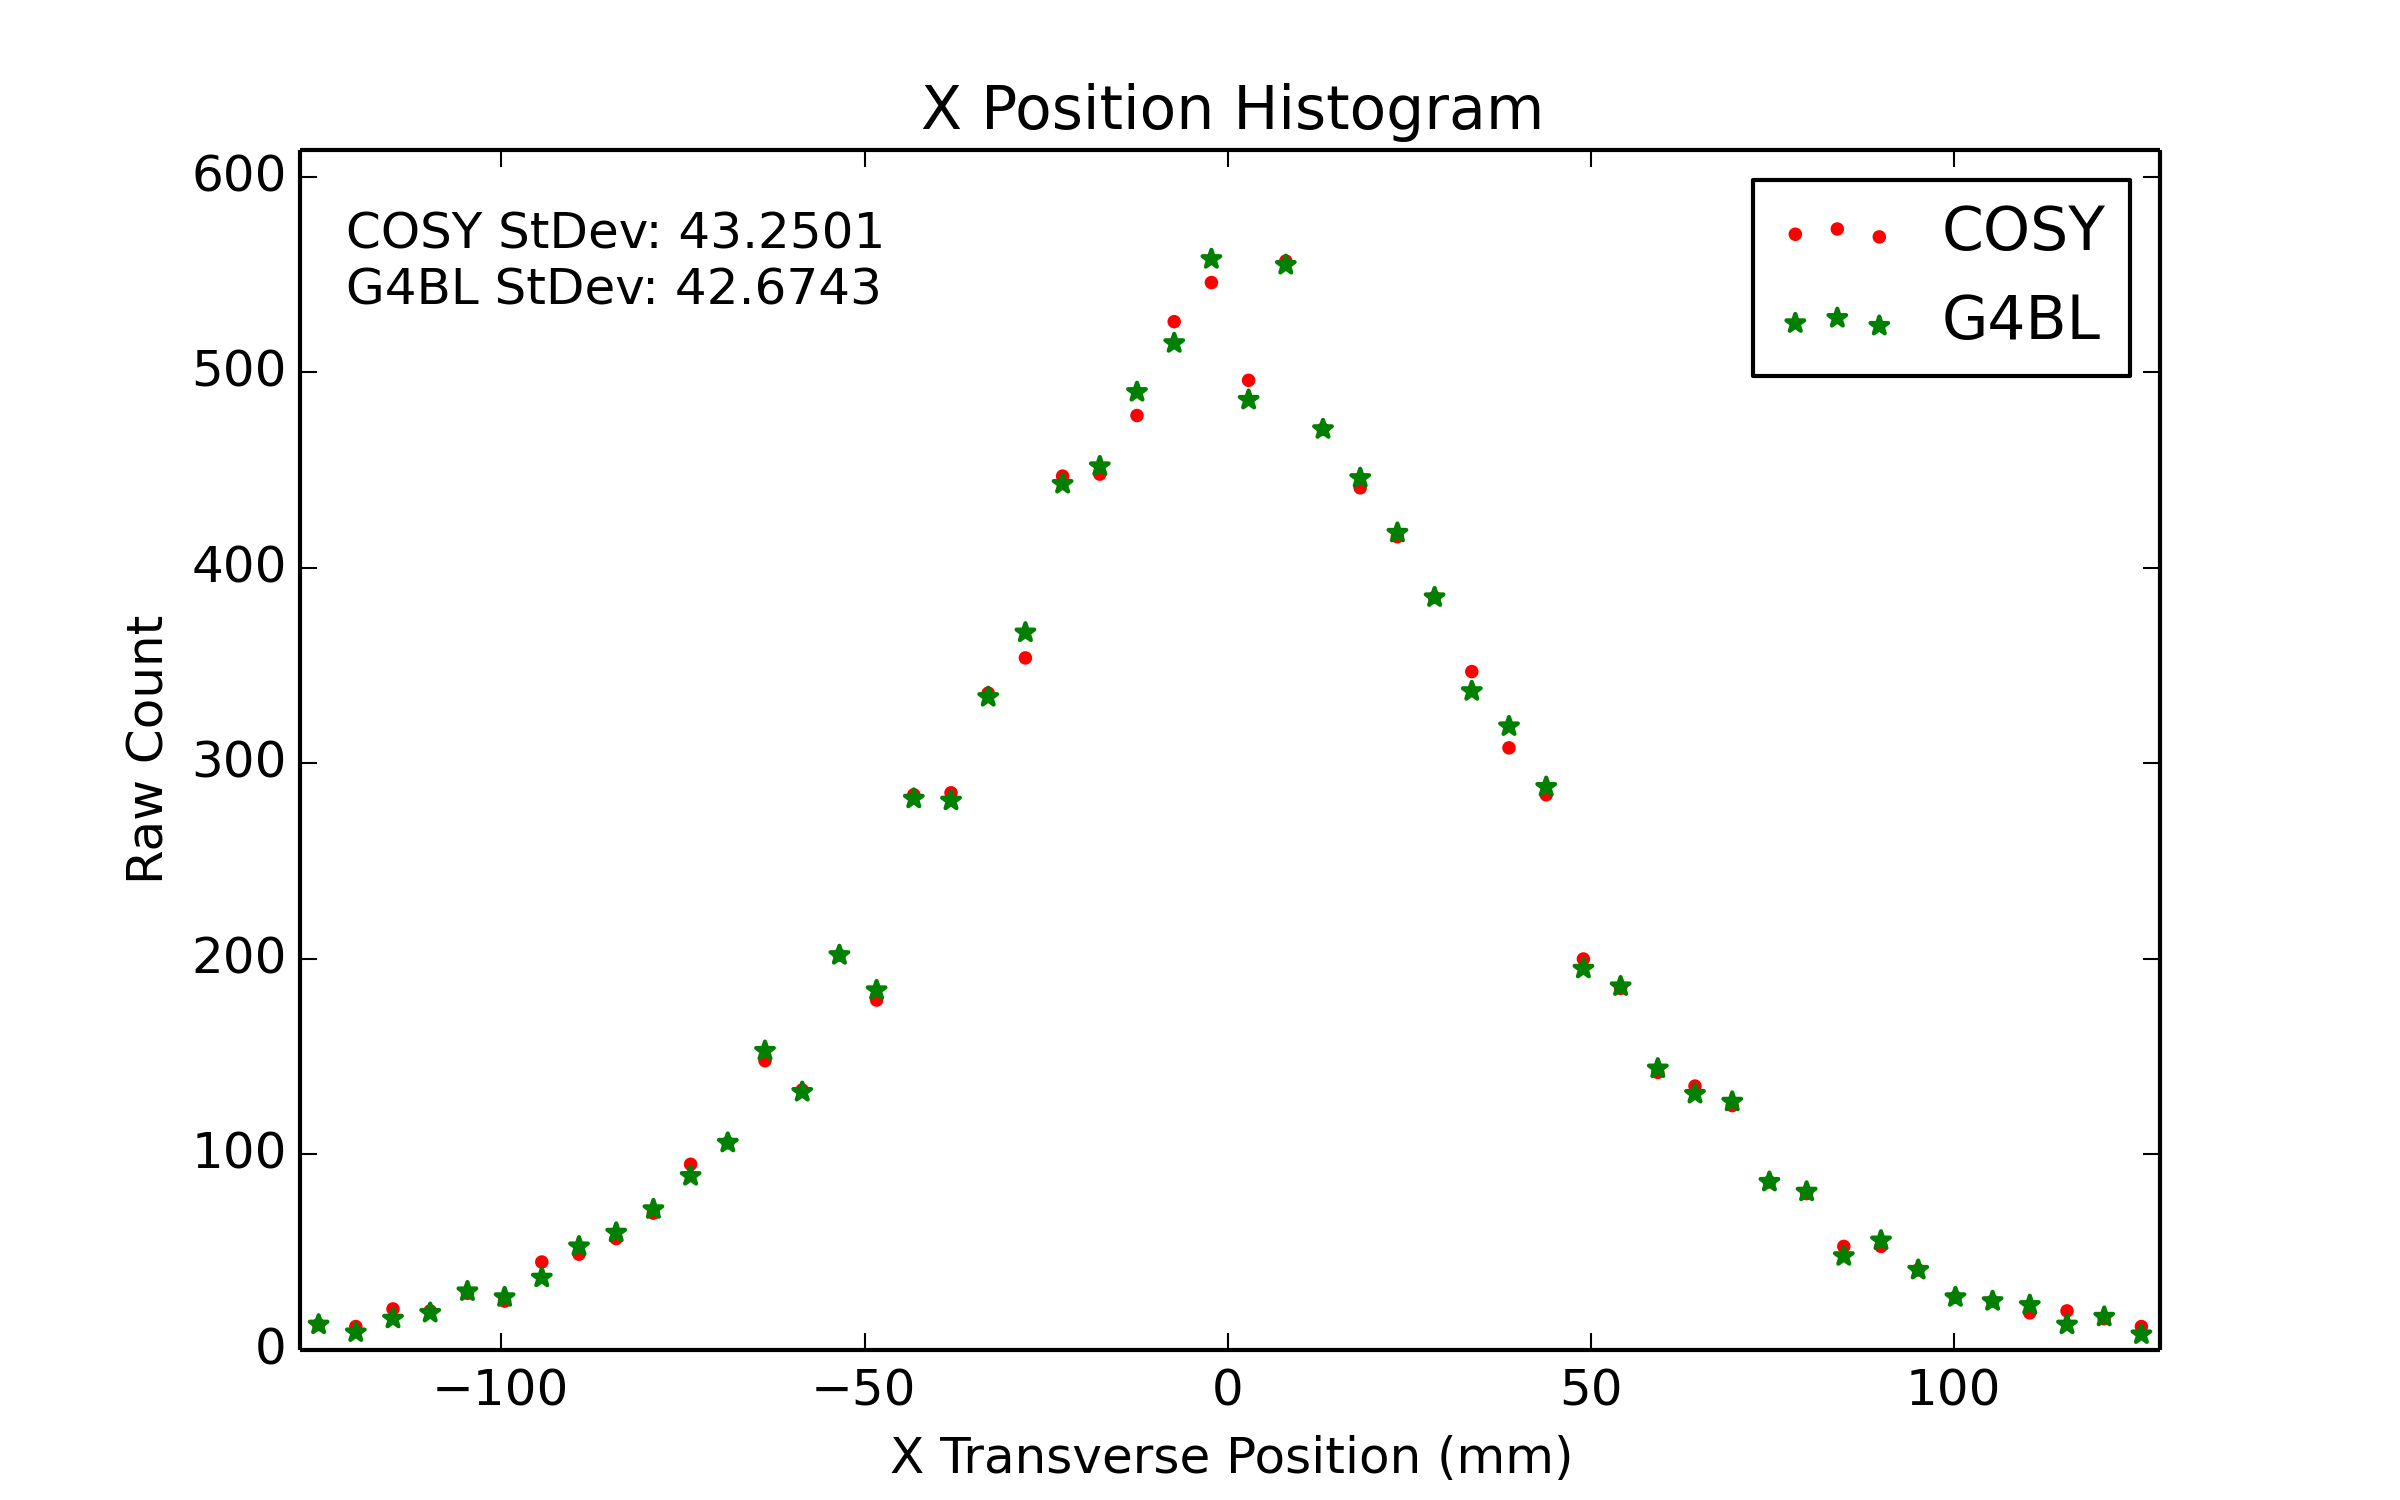
\includegraphics[width=\columnwidth]{xposition.png}
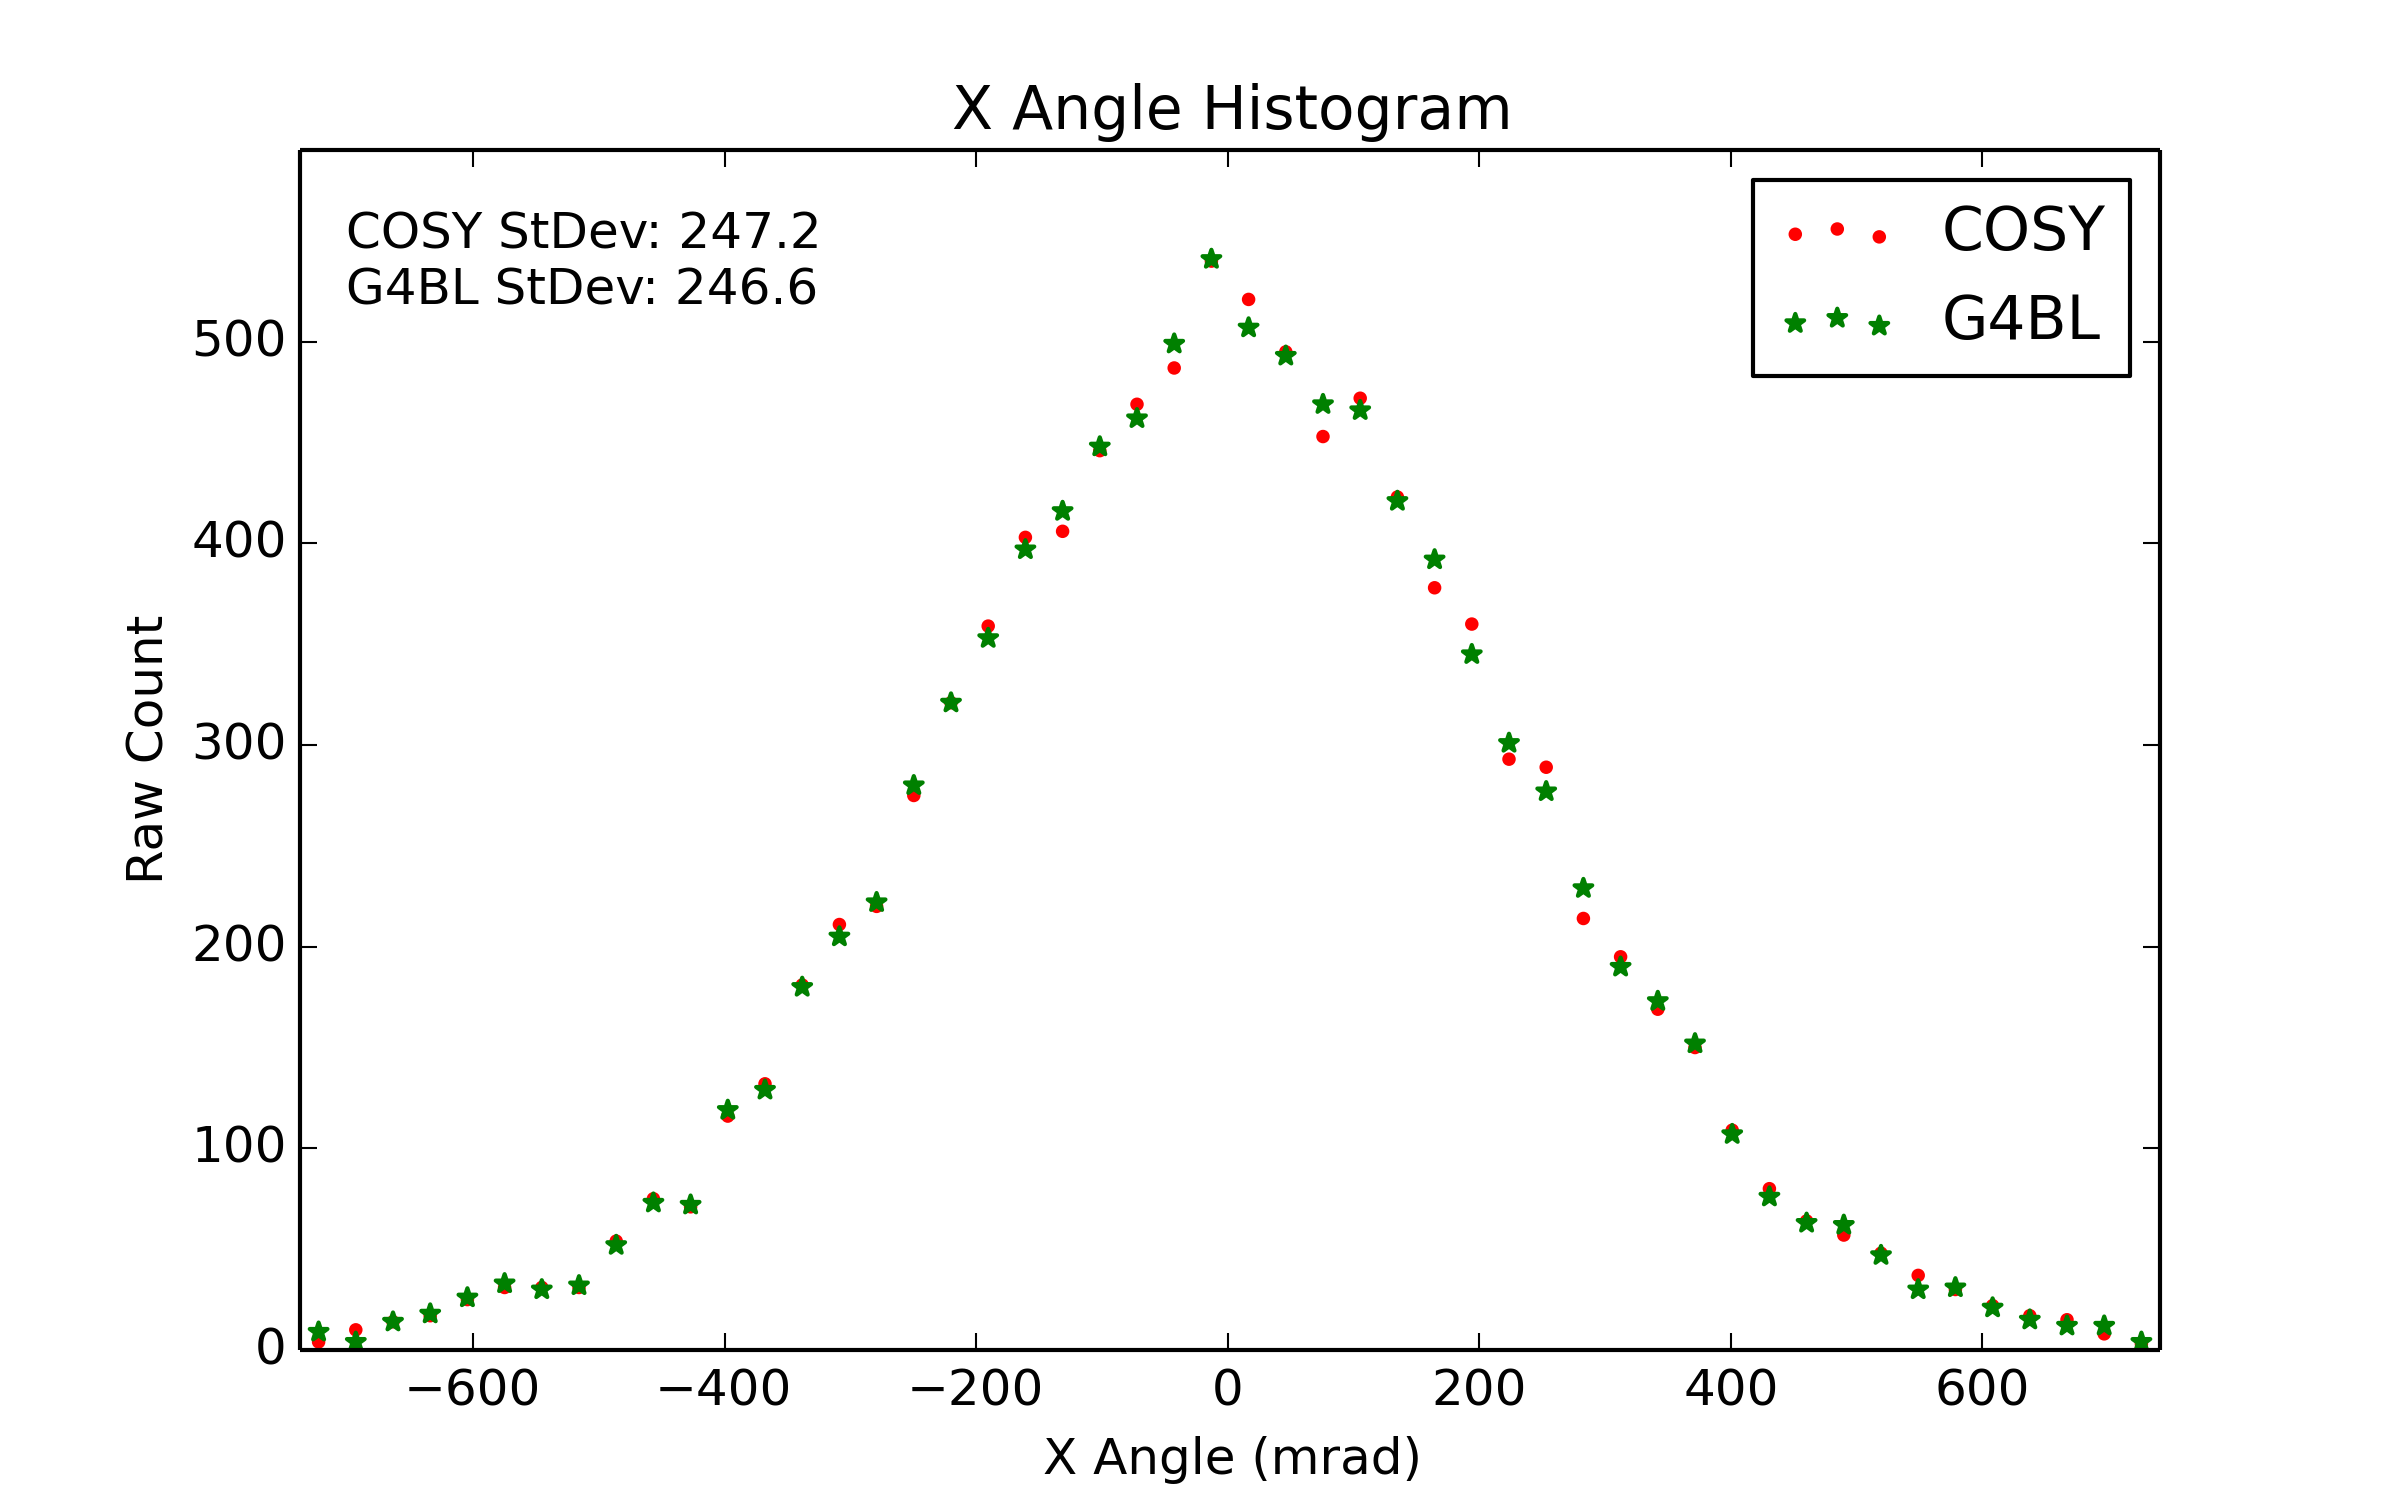
\includegraphics[width=\columnwidth]{xangle.png}
\caption{Final position and angle histogram comparison between COSY and G4beamline, magnetic coils only.}
\label{fig:mice_coil_histograms}
\end{figure}

For the flat lithium hydride absorber, the simulation in G4Beamline was carried out using the \texttt{tubs} routine. In COSY, the newly implemented routine \texttt{ABSPOLY} (polynomial absorber) was used. Details on the stochastic processes implemented by \texttt{ABSPOLY} can be found in \cite{ipac2015}. The results are summarized in Figure~\ref{fig:mice_coil_absorber} and are in excellent agreement between the two codes.

\begin{figure}[!ht]
\centering
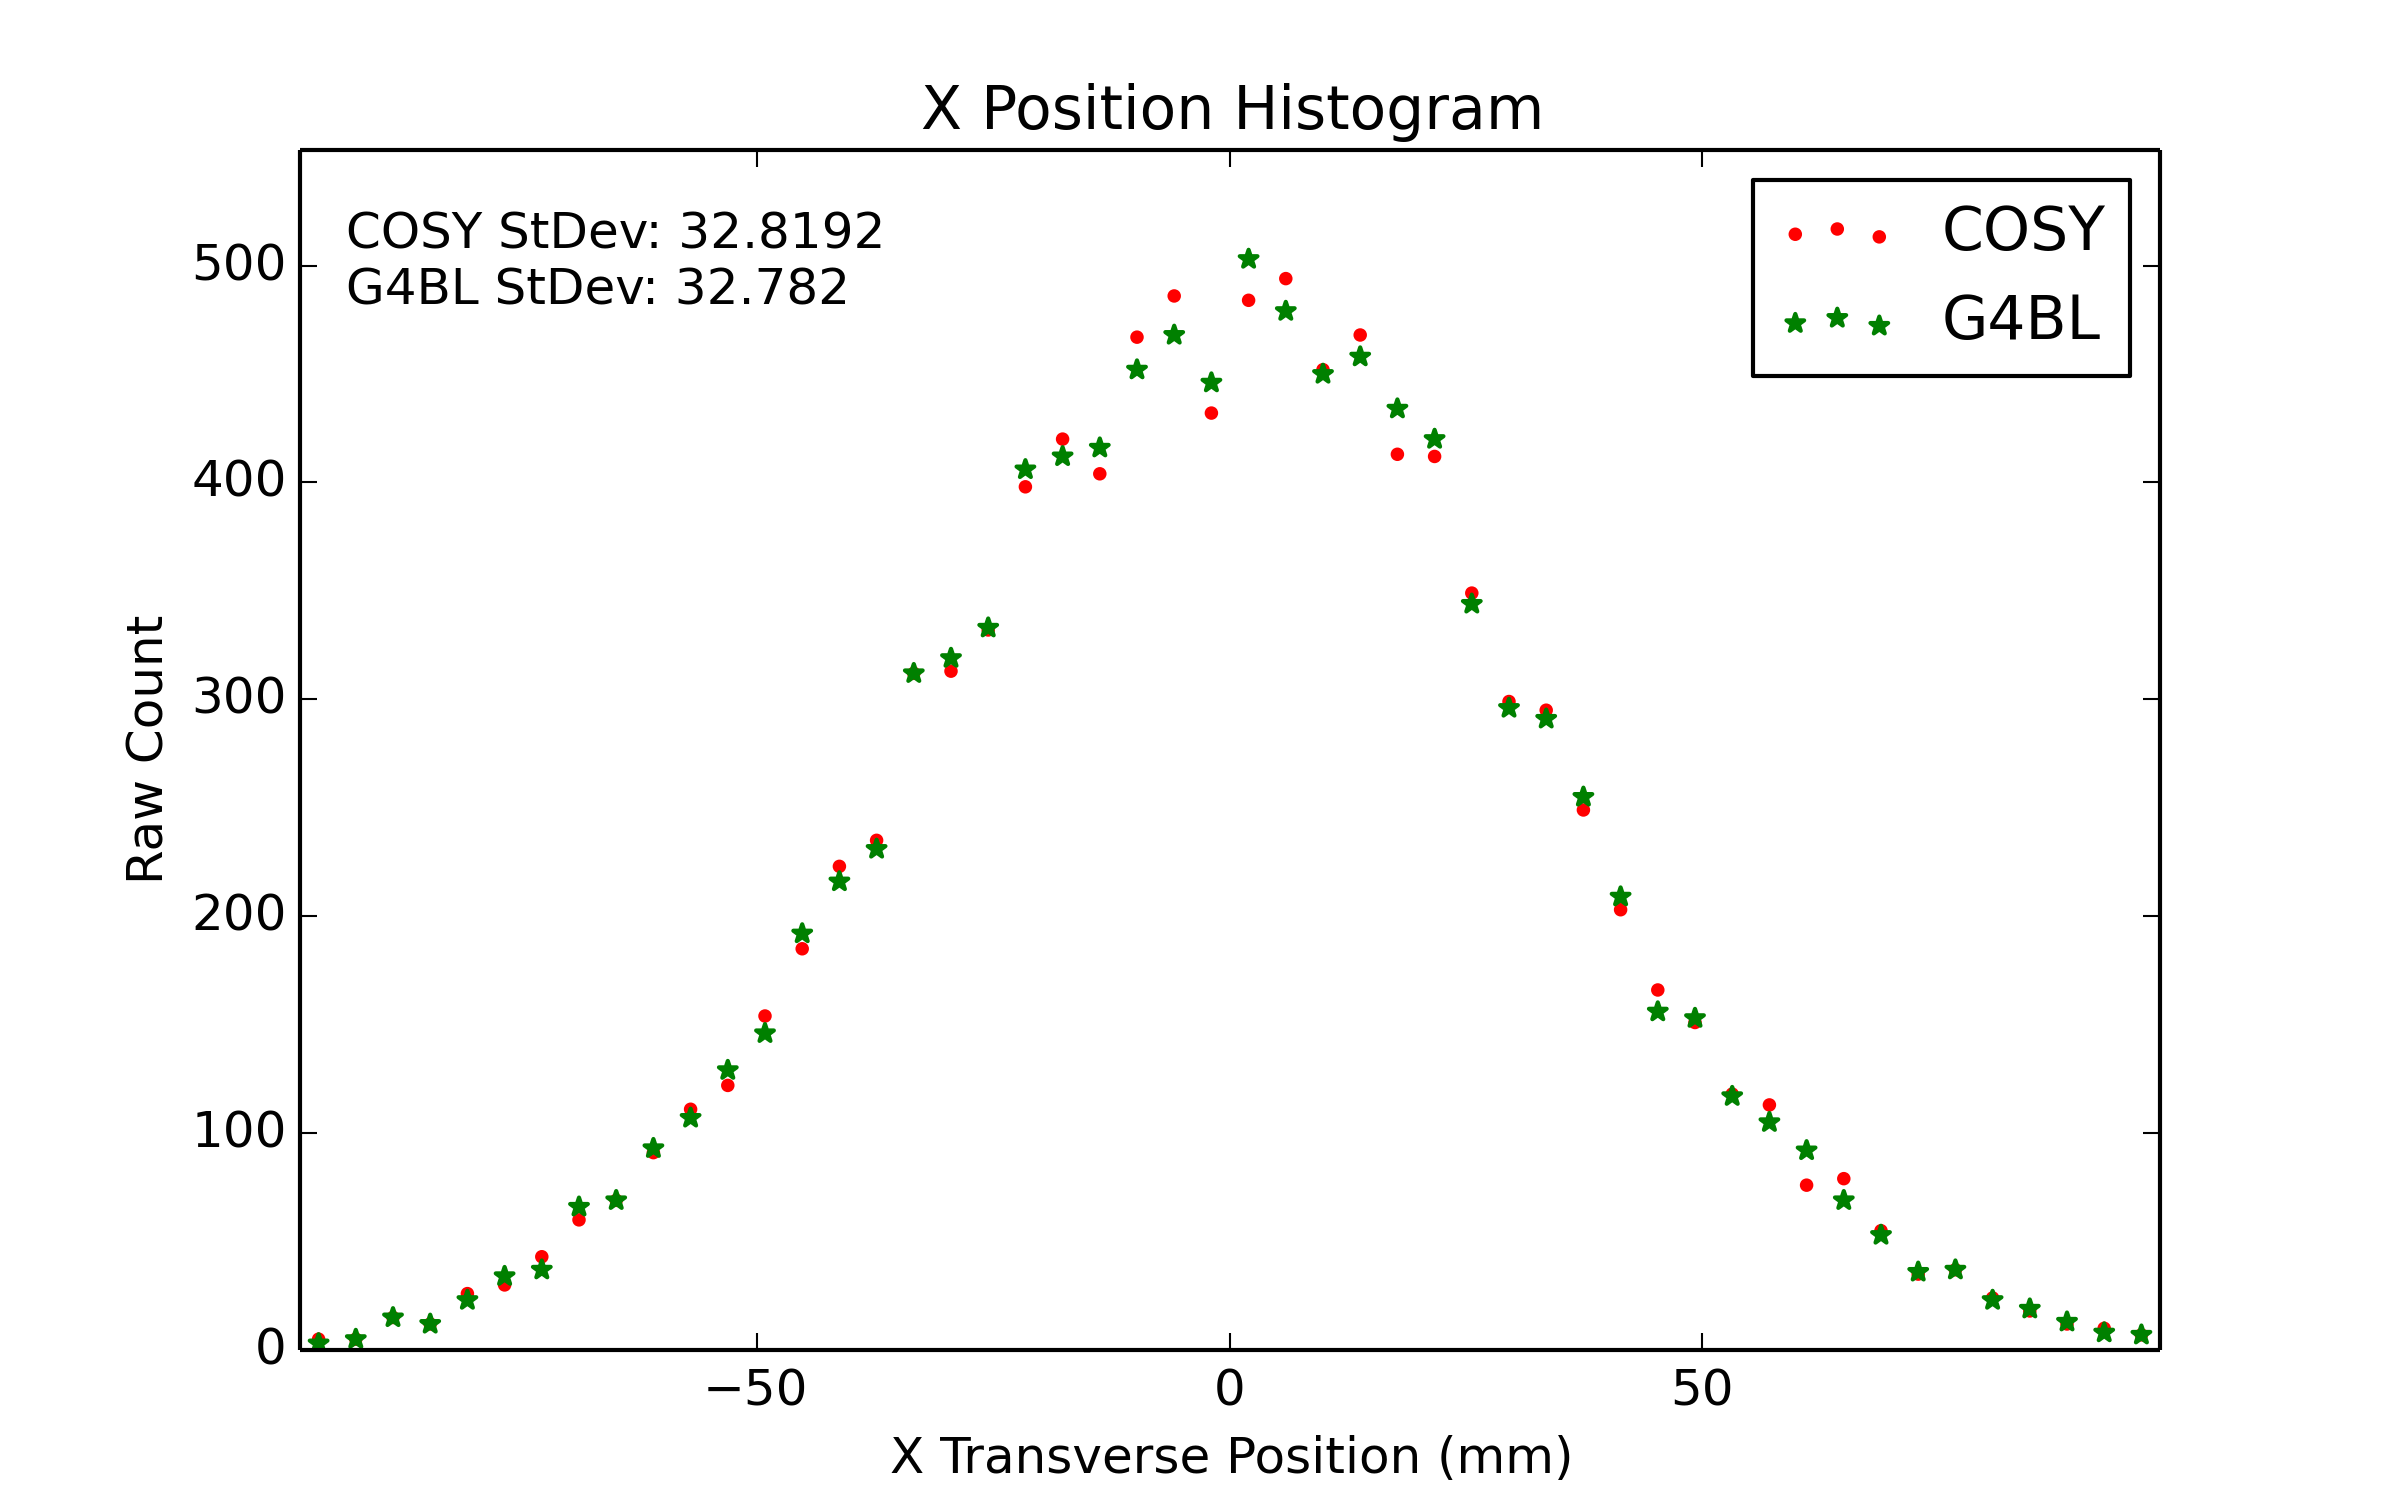
\includegraphics[width=\columnwidth]{LiH_xposition.png}
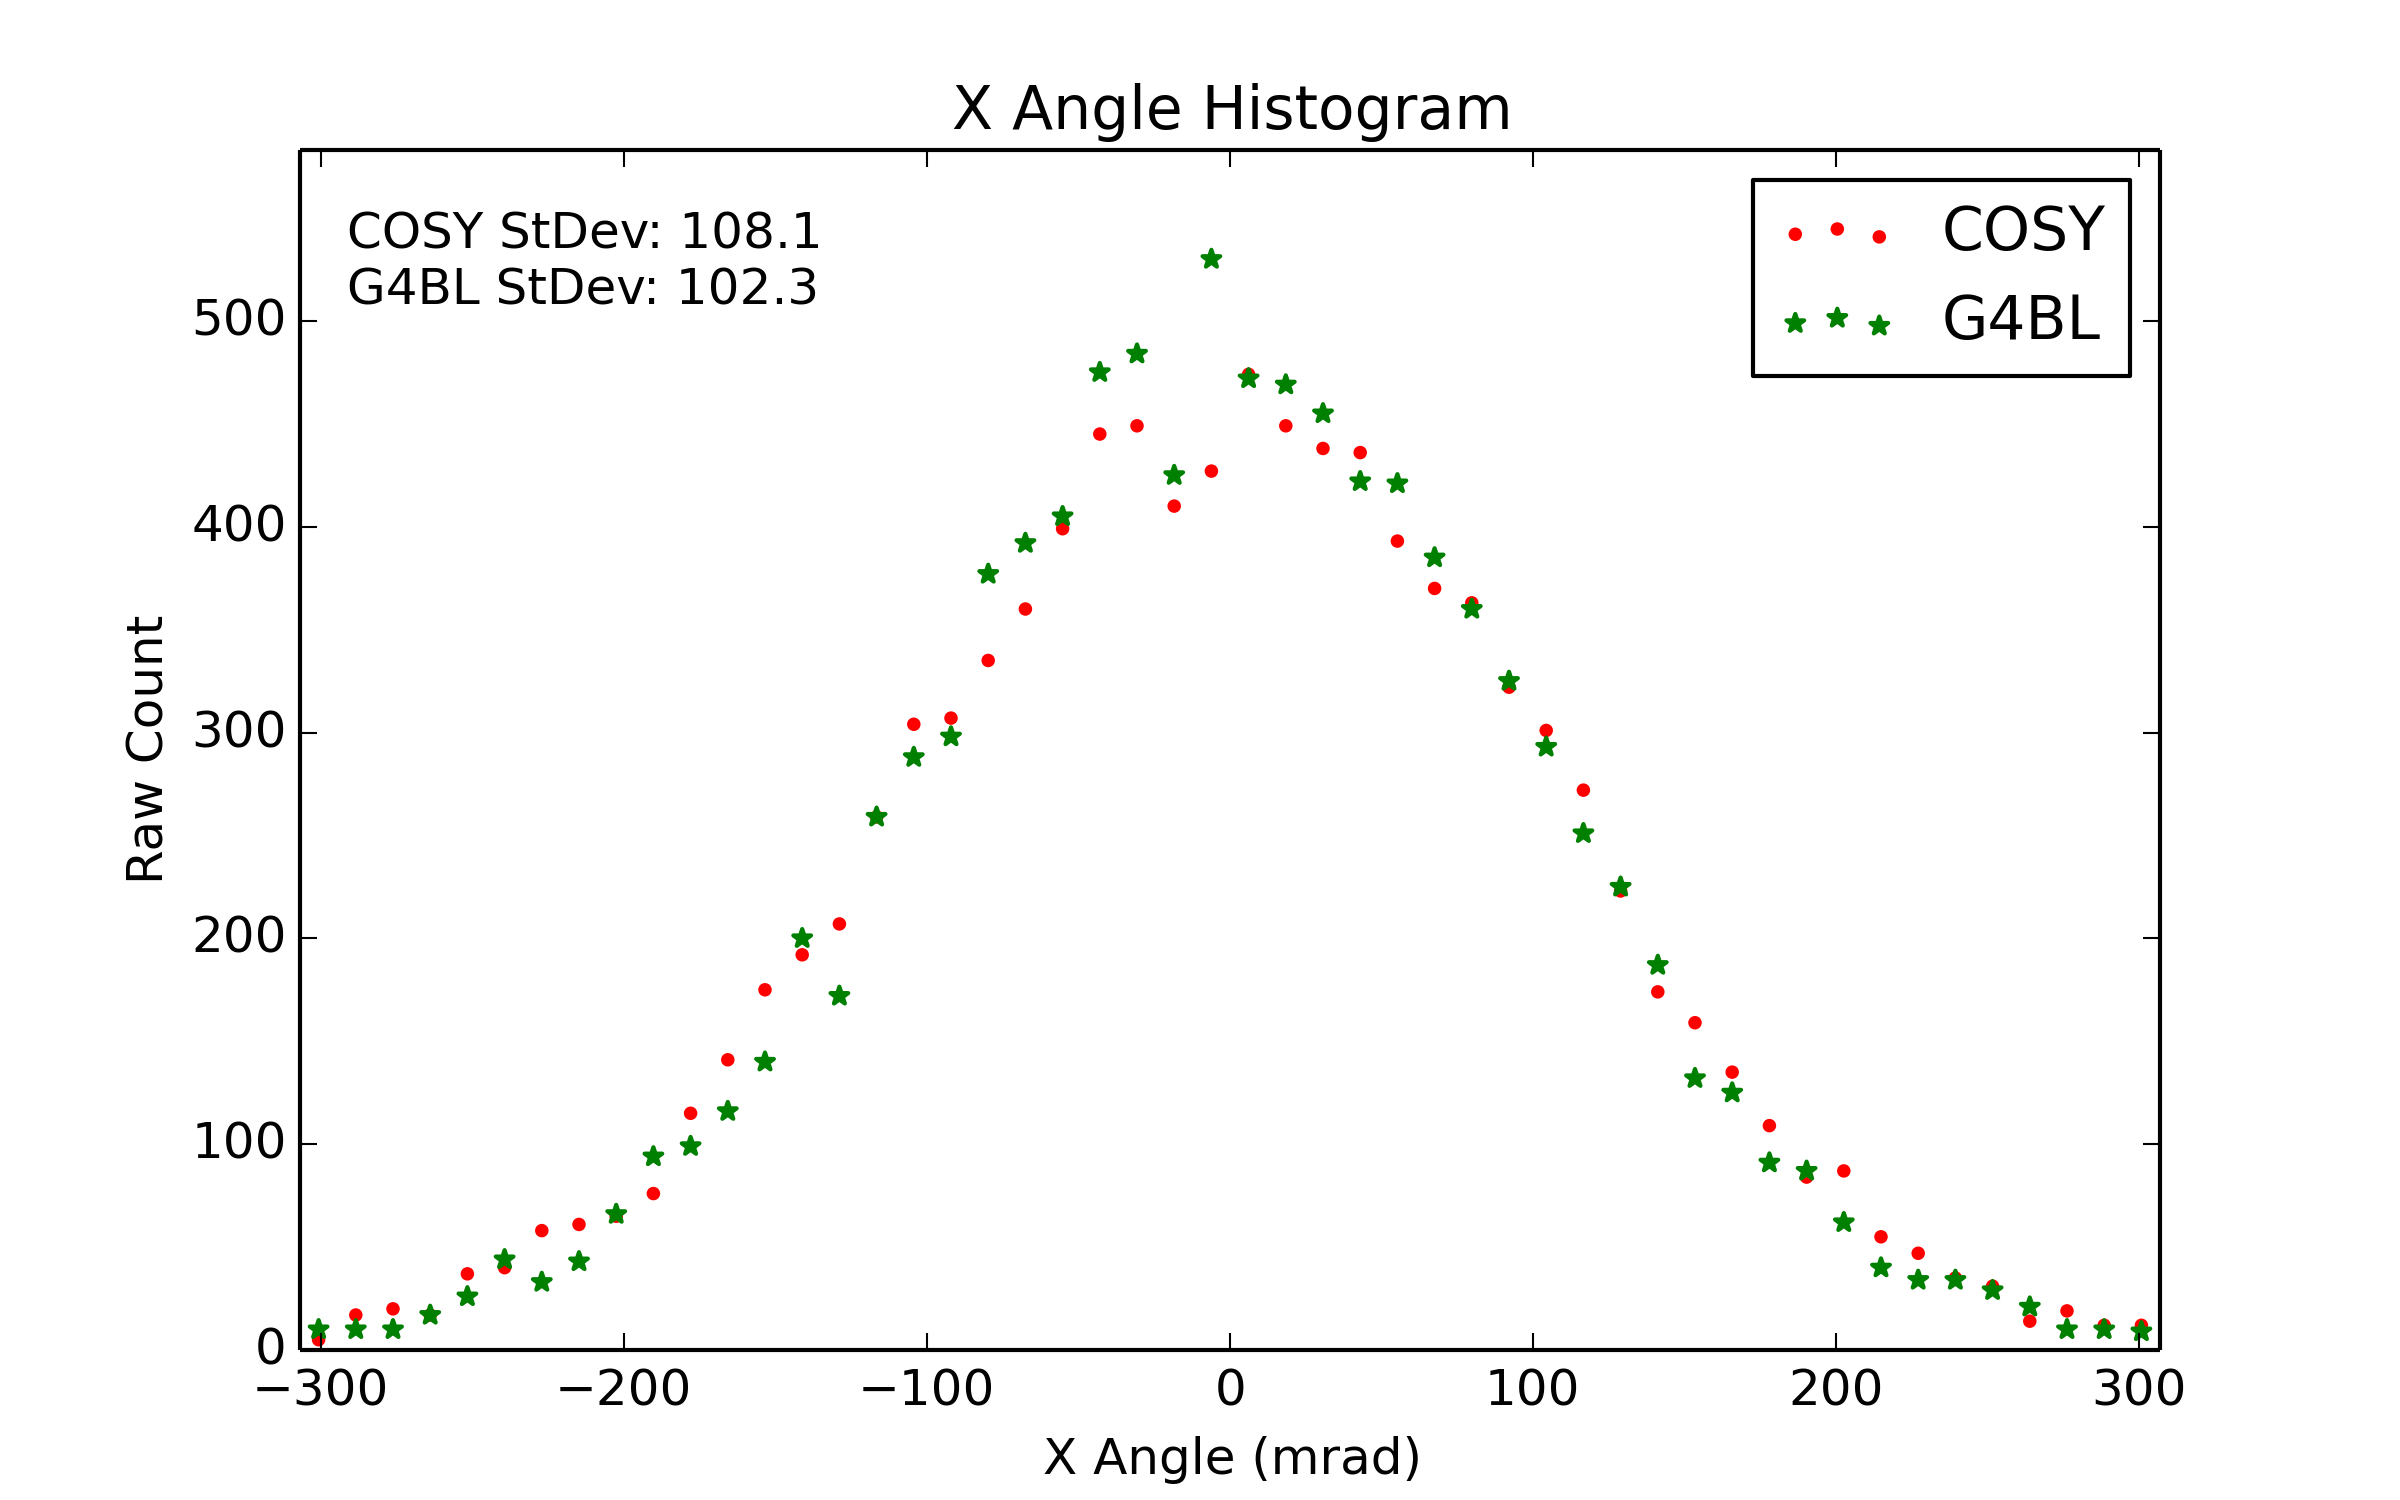
\includegraphics[width=\columnwidth]{LiH_xangle.png}
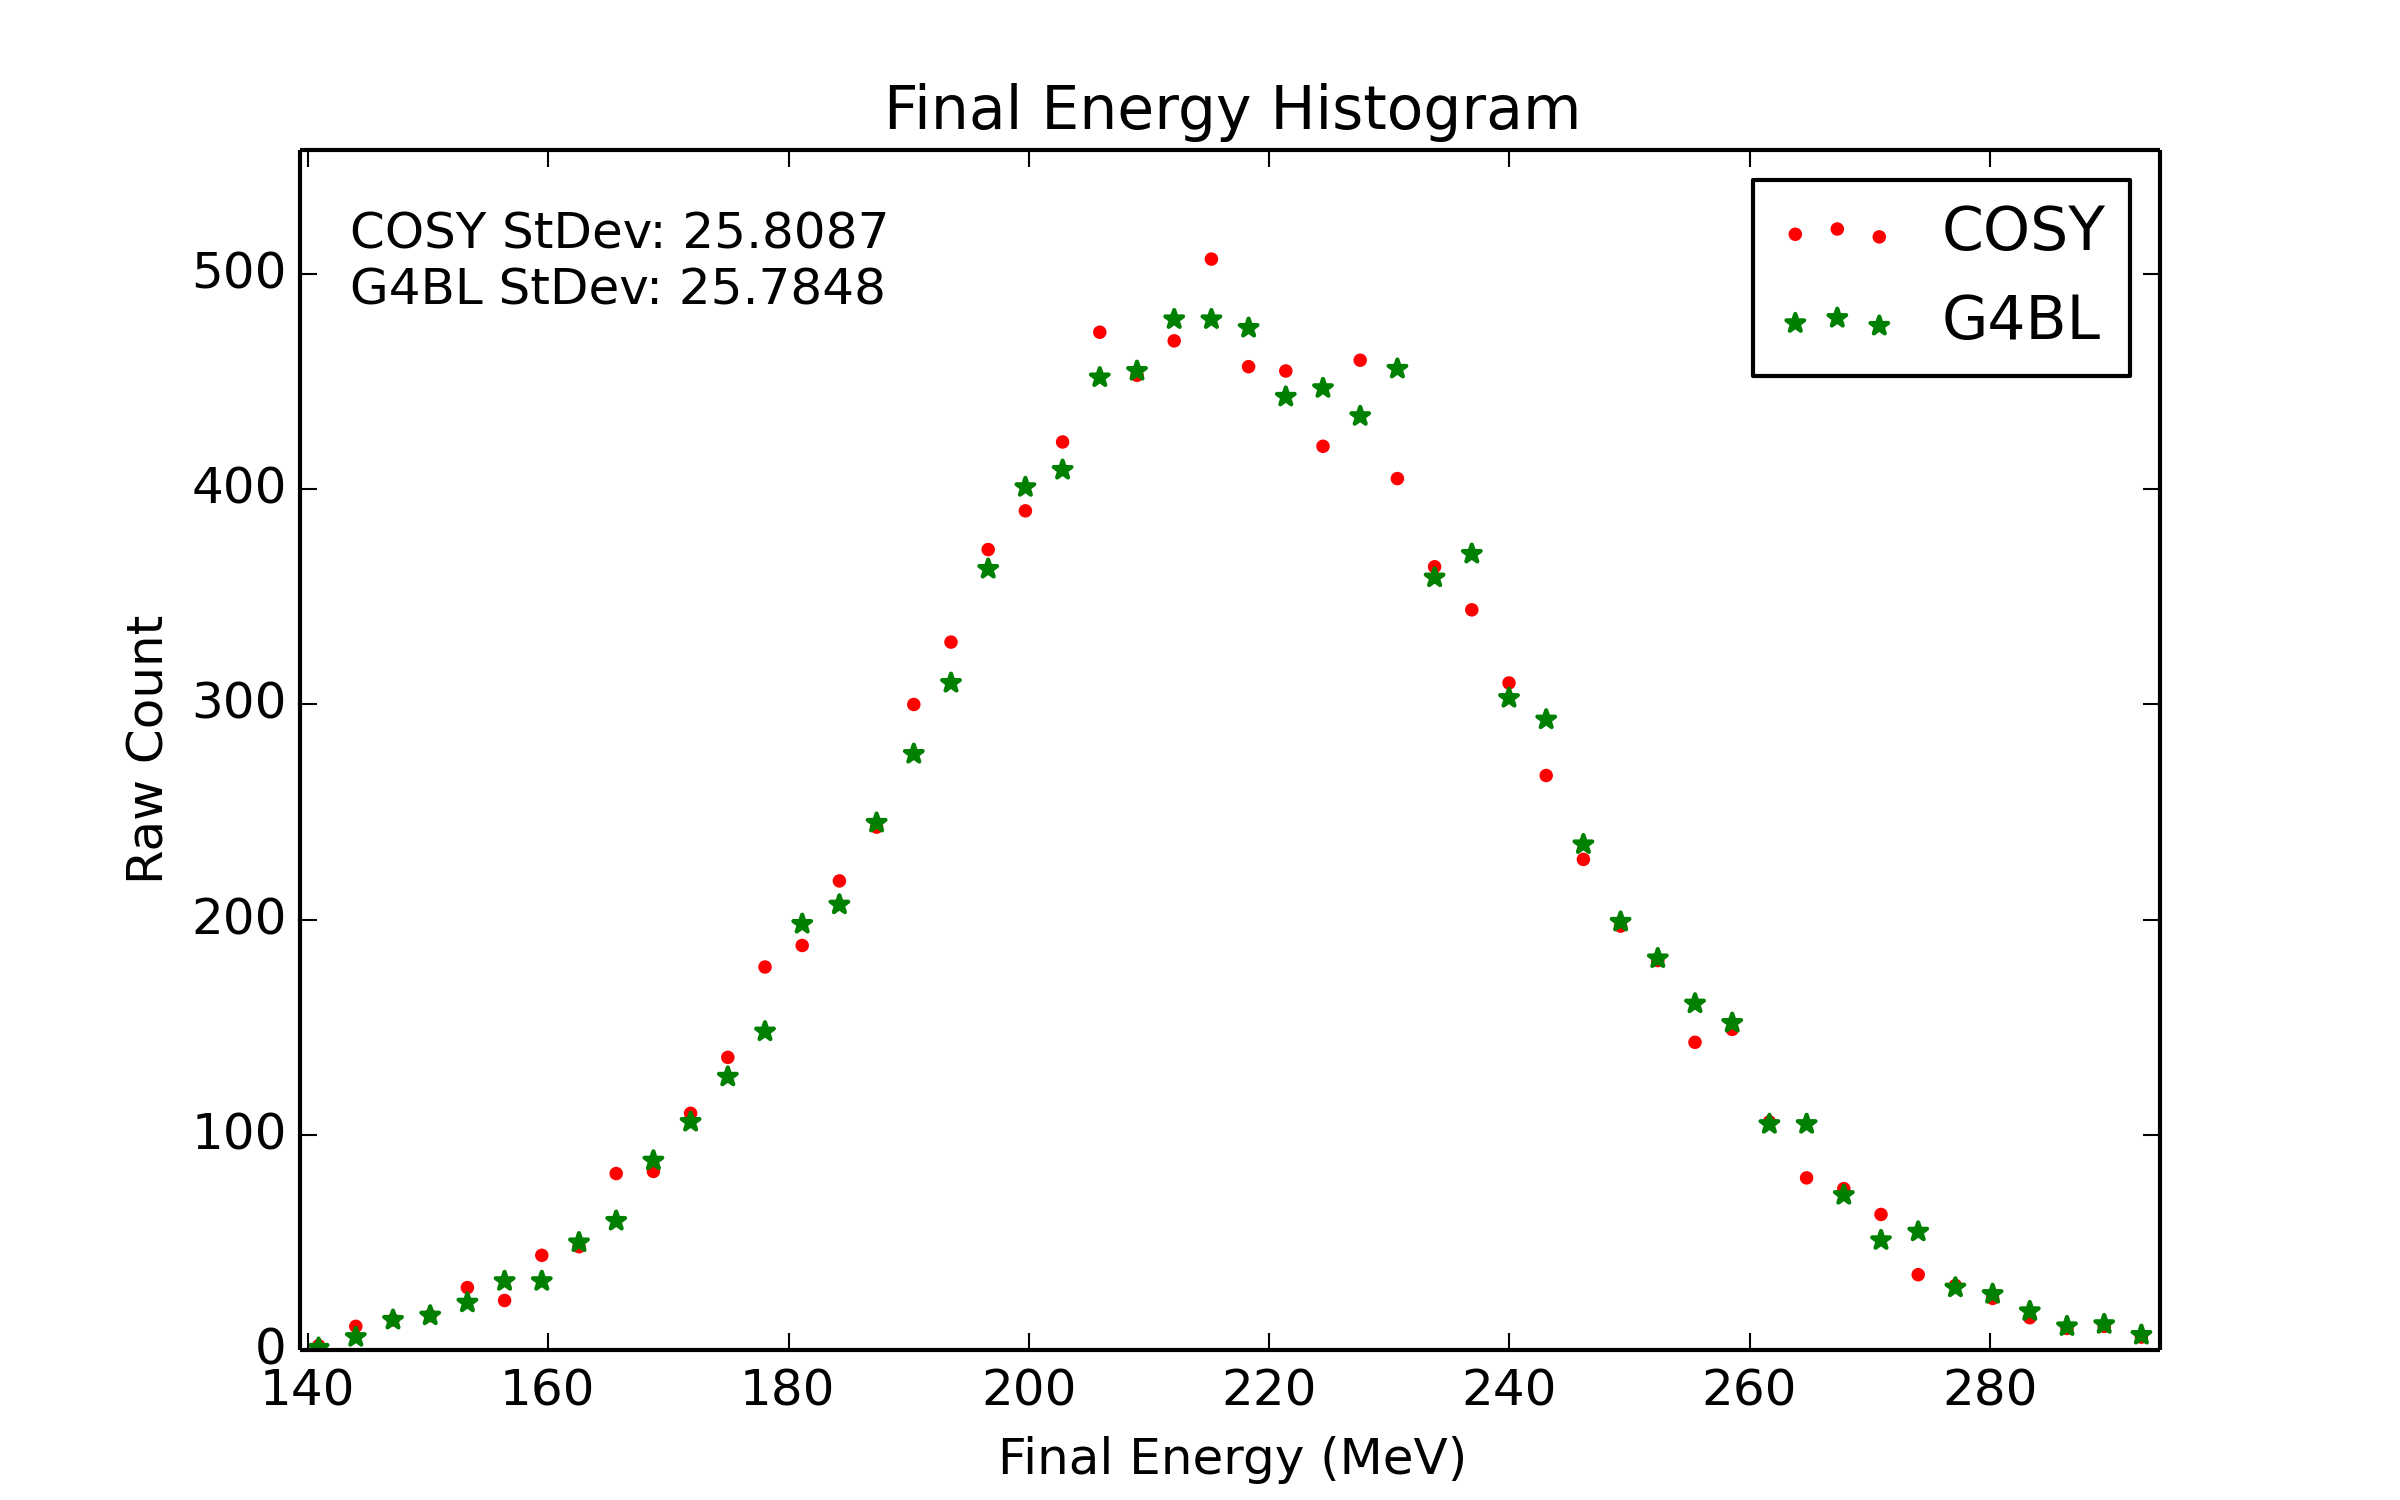
\includegraphics[width=\columnwidth]{LiH_energy.png}
\caption{Final position, angle, and final energy histogram comparison between COSY and G4beamline, LiH absorber only.}
\label{fig:mice_coil_absorber}
\end{figure}

\section{Current Challenges}
While there is a good agreement between COSY and G4beamline as far as the absorbers and the coils are considered separately, the study of the results of combining the two is underway. Additionally, some configurations use tilted coils. These coils generate dispersion, which in conjunction with the wedge absorber could provide emittance exchange required for full six-dimensional cooling as opposed to the transverse cooling. However, COSY does not currently have a way to arbitrarily tilt an arbitrary arrangement of coils, and so such functionality needs to be implemented and adopted. Finally, the differences in the COSY RF kick versus the G4Beamline pillbox model need to be explored and addressed. This could potentially result in implementing a new lattice element in COSY.

\bibliography{bib}{}
\bibliographystyle{unsrt}
\mbox{}
\end{document}